\section{Microservice Architecture}
\label{se:microservice}

A microservice architecture style is an approach to developing a single application as a package of small services, each working in their process and communicating using lightweight mechanisms, often through the delivery of a \acrfull{rest} \acrshort{api}. These services are built around commercial capacities and can be used independently by fully automated implementation machines \cite{LewisMicroservices}. In a microservice architecture, each microservice implements decoupling from other microservices and minimizing the centralized dependencies. Thus, we can use different programming languages and data storage technologies to implement each microservice.

There are lots of microservice patterns developed and evolved. Through the following sections, we will discuss some of the microservice design patterns mostly used in the context of designing the software architecture for our research in brief. Next, we will discuss how microservice architecture promotes only to create endpoints that solely belong to each service logical domain. Next, consider only using a database per service, which allows it to be loosely coupled between systems and achieves high scalability. Then we will discuss how distributed transactions can makeover microservices. Last, we will discuss a concept called \emph{the scale cube}, which explains the scalability from the perspective of x-axis, y-axis, and z-axis.


%%%%%%%%%%%%%%%%%%%%%%%%%%%%%%%%%%%%%%%%%%%%%%%%%%%%%%%%%%%%%%%%%%%%%%%%%%%%%%%%
\subsection{Smart Endpoints and Dumb Pipes  Microservice Pattern}
\label{subse:dumb_pipes}

When building communication endpoints, many architectural approaches are adding significant smart by providing different protocol supports and complex logic support through the endpoints. As an example, \acrshort{esb} supports multiple protocols, and endpoints can be used to implement complex logic. But microservice architecture follows an alternative approach called as \emph{Smart endpoints and dumb pipes} \cite{LewisMicroservicesPipes}. Applications built based on microservice architecture are intended to be as disconnected and as coherent as possible. Each microservice has its domain logic and independent of other microservices logic and works more like filters in the classical Unix pipelines. Each microservice provides its functionalities as a \acrshort{rest} \acrshort{api} instead of using complex protocols. After receiving a request for each microservice through its \acrshort{rest} \acrshort{api}, it applies the correct logic and produces a response.

%%%%%%%%%%%%%%%%%%%%%%%%%%%%%%%%%%%%%%%%%%%%%%%%%%%%%%%%%%%%%%%%%%%%%%%%%%%%%%%%
\subsection{Database per Microservice Pattern}
\label{subse:database_per_service}

\acrshort{microservice} prefers to have each microservice manages its database, either different instances of the same database technology or entirely different database systems - an approach called \emph{Polyglot Persistence} \cite{LewisMicroservicesManagement}.

The idea is to keep the persistent data of each microservice private for this service and only to make it accessible through an \acrshort{api}.
There are different ways to keep the permanent data of a microservice private. But it is not required to set up a database instance for each microservice. For example, when you use a relational database, the following methods can be used to keep the data private \cite{RichardsonMicroservicesService}:
\begin{itemize}
    \item Individual tables per service -- each microservice has a set of tables that restricts access for other microservices.
    \item Schema per service -- each service has a private database schedule for a given microservice.
    \item Database server per service -- each service has its database server.
\end{itemize}

\emph{Private tables per service} and \emph{schema per service} have the lowest overhead. The use of a schema per service is interesting because it makes the property clearer. Some high throughput services may require their database server.

%%%%%%%%%%%%%%%%%%%%%%%%%%%%%%%%%%%%%%%%%%%%%%%%%%%%%%%%%%%%%%%%%%%%%%%%%%%%%%%%
\subsection{Distributed Transactions over Microservices Pattern}
\label{subse:sagas}

Every microservice can have its database to guarantee a loose couple between microservices. Maintaining data consistency between services is a challenge because two phase-commit/distribution transactions are not an option for many applications. To archive distributed transactions, a service publishes an event when the data changes. Other services use this event and update their data \cite{RichardsonMicroservicesSagas}. The above approach is also called the \emph{Saga pattern}.

%%%%%%%%%%%%%%%%%%%%%%%%%%%%%%%%%%%%%%%%%%%%%%%%%%%%%%%%%%%%%%%%%%%%%%%%%%%%%%%%
\subsection{The Scale Cube Concept}
\label{subse:scale_cube}

The scalability of a system can be explained via a concept called \emph{the Scale Cube}, which talks about the scalability of the application by defining over X, Y, and Z axes.

\paragraph{X-axis scaling} -- When scaling an application through the x-axis, multiple instances of the application execute behind a load balancer. If there are \textit{n} copies, then each copy handles 1/\textit{n} of the load. The above simple approach is commonly to scale a service.

\paragraph{Y-axis scaling} -- When compared to the z-axis and x-axis scaling, which follows the concept of running multiple identical copies of the application, but y-axis scaling segregates the application into multiple services in the same domain. So, the end services are responsible for one or more closely related functions of the previous service before the segregation. There are different ways to split the application into services.
\begin{itemize}
    \item Verb-based decomposition. e.g., checkout.
    \item Decompose the application by the noun. e.g., order management.
    \item It is possible to use a combination of verb-based and noun-based decomposition for an application.
\end{itemize}
The microservice architecture is an application of y-axis scaling.

\paragraph{Z-axis scaling} -- The z-axis scaling follows the concept of each service running the same application code (similar to x-axis scaling). The big difference is that each service is responsible for only a subset of the data. z-axis splits are commonly used to scale databases. As an example, data partition (aka., sharded) across a set of servers based on an attribute of each record.
Even our research is a design based on the y-axis scaling; it is possible to use the z-axis scaling to further scaling the system. We will discuss more detail in \cref{se:discussion}.


%%%%%%%%%%%%%%%%%%%%%%%%%%%%%%%%%%%%%%%%%%%%%%%%%%%%%%%%%%%%%%%%%%%%%%%%%%%%%%%%
\subsection{WDIAS Microservices}
\label{sebse:wdias_microservices}

\cref{fi:wdias_micro_on_demand} and \ref{fi:wdias_micro_async} show the system interaction of the WDIA microservices architecture while handling requests. Each circle in the figures represents a microservice in the \acrshort{wdias}. And each microservice is implemented as a containerized application. The left side of \cref{fi:wdias_micro_on_demand} shows the import modules of the \acrshort{wdias}, and the right side shows the export modules. Also, we implemented each module as a microservice to independent maintainability and upgradability. We followed the concept of smart endpoints and dumb pipes explained in \cref{subse:dumb_pipes}, and each import microservice only does the specific task of converting and forwarding the request to the correct data adapter module. For scalar, vector, and grid data types, we created adapter microservices that are optimized for storing such kinds of data. The metadata data of the timeseries store using an RDBMS, which gives more performance over retrieving timeseries metadata. The metadata is cached using an in-memory database to fast access while implementing the database structure. The system generates a unique identifier for each timeseries, and throughout the \acrshort{wdias} system, all microservices use it to handle data for fast access.

\begin{figure}[htp]
    \centering
    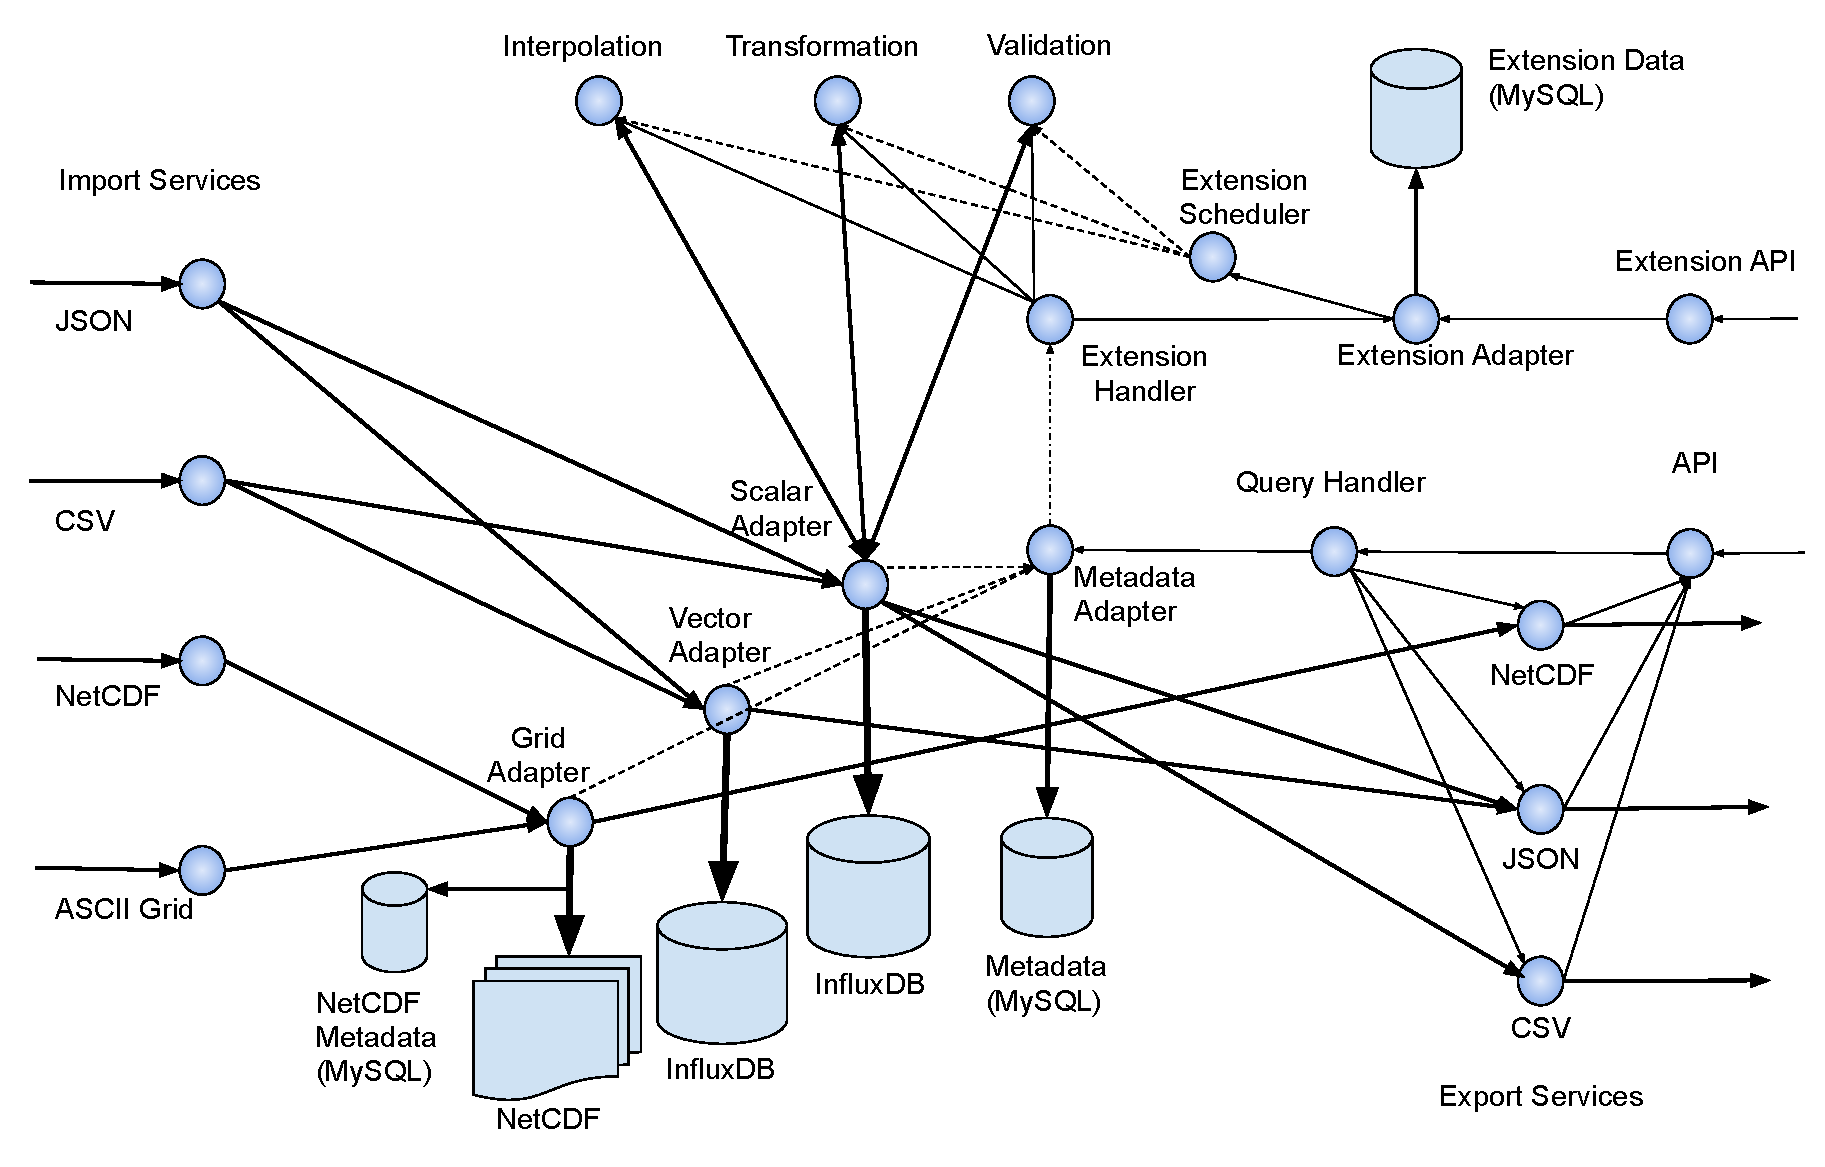
\includegraphics[width=1\textwidth]{method/microservice/microservice_architecture-handle_on_demand-v4.pdf}
    \caption{\acrshort{wdias} architecture for handling requests on demand.}
    \label{fi:wdias_micro_on_demand}
\end{figure}

Export module microservices also follow the concepts of single responsibility and provide the capability to export the data into required formats of the weather models. Each data type adapter follows the microservice architecture concept of database per service, as mentioned in \cref{subse:database_per_service} When the system requires more database throughput, it is easy to scale each database instance by adding more resources or using z-axis scaling concepts.

\begin{figure}[htp]
    \centering
    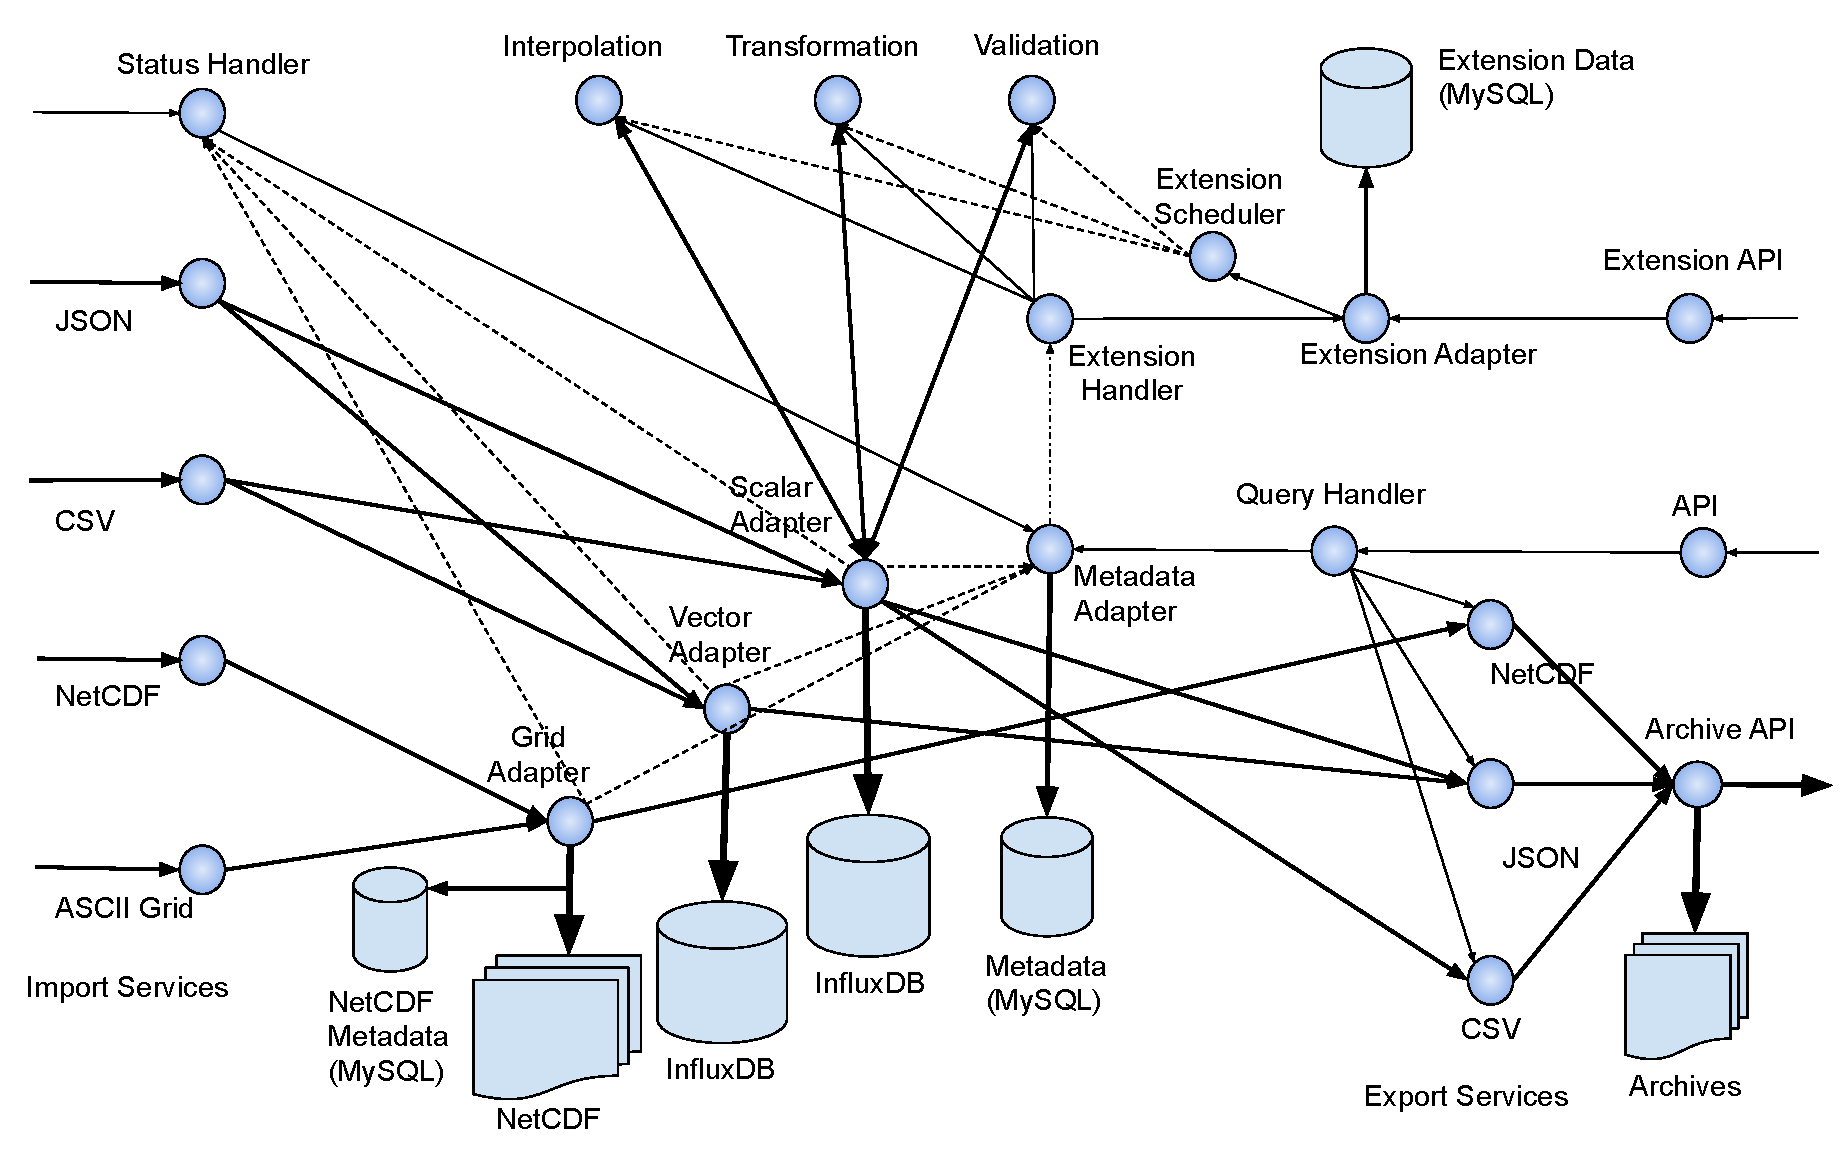
\includegraphics[width=1\textwidth]{method/microservice/microservice_architecture-handle_on_async-v4.pdf}
    \caption{\acrshort{wdias} architecture for handling requests asynchronously.}
    \label{fi:wdias_micro_async}
\end{figure}

As shown in \cref{fi:wdias_micro_on_demand}, when a request with a smaller payload comes to the system, the system handles the request on-demand and response back. However, as shown in \cref{fi:wdias_micro_async}, when a request with a larger payload comes to the system, it stores the data for an asynchronous process and responds with a unique id that can be used to verify whether data processed successfully or not. We used the microservice concept of Saga, as mentioned in \cref{subse:sagas}, while processing the grid data. First, it stores the data and responds with a unique identifier to the user. After successfully storing the data, the microservice publishes an event. Another microservice listens to those events and processes the data and updates the system status.

\begin{figure}[htp]
    \centering
    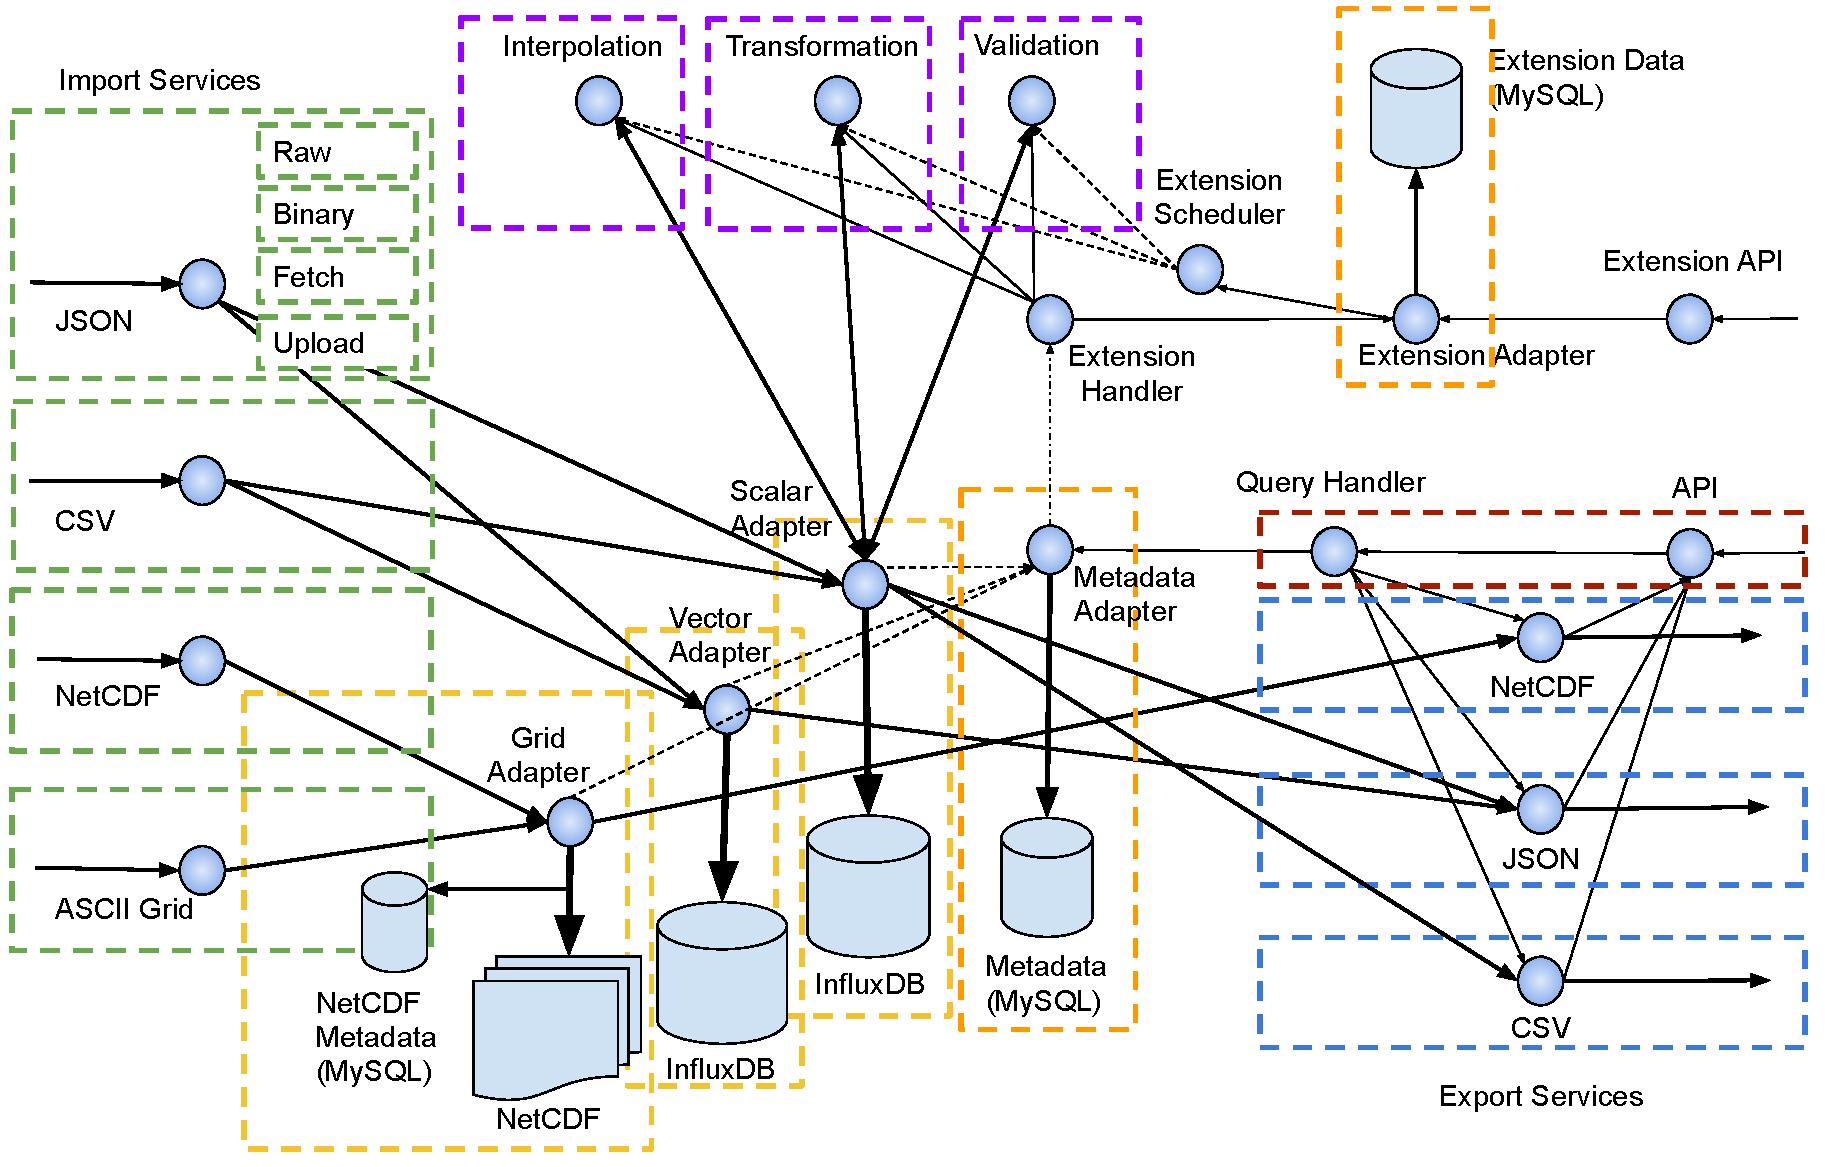
\includegraphics[width=1\textwidth]{method/microservice/separation_microservices-v4.pdf}
    \caption{Separation of \acrshort{wdias} microservices.}
    \label{fi:wdias_micro_separation}
\end{figure}

\cref{fi:wdias_micro_separation} shows the clear separation of microservices into the modules of the \acrshort{wdias}. Each adapter has a separate database, and the database is hosted separately for the high performance and to avoid interference.
Apart from that, as we further discuss in \cref{se:data_preprocess}, the extension modules are running independently, such as Interpolation, Transformation, and Validation, and we will also discuss in \cref{se:data_preprocess}. The Extension Adapter allows users to register new event-based or time-based triggers for the extensions. The extension scheduler triggers the events based on time and the extension handler triggers events based on data change.


%%%%%%%%%%%%%%%%%%%%%%%%%%%%%%%%%%%%%%%%%%%%%%%%%%%%%%%%%%%%%%%%%%%%%%%%%%%%%%%%
\subsection{WDIAS Application Programming Interface}
\label{sebse:wdias_api}

We defined an \acrshort{rest} as the communication layer for \acrshort{wdias}, and it affects the microservice architecture design as well. It follows a simple \acrshort{rest} \acrshort{api} and allows users to interact with the system through HTTP methods.

We provided a set of timeseries endpoints to register new timeseries metadata before storing the real data, and a detailed description appears in Appendix A. Timeseries endpoints allow users to interact with Metadata Adapter to create and update the timeseries metadata. After creating timeseries metadata, we cached on the Query Handler to perform search queries and geo-indexed to support geo-based queries. When a user registers a timeseries metadata, the system generates a unique timeseries identifier based on the metadata values. Then the user can use that identifier to store the real weather data and retrieve stored data.

Current \acrshort{wdias} only supports handling point locations and grid locations. If it needs to extend the system to store irregular grid data, then it should add another set of location endpoints for storing irregular grid location details.

Other than the endpoints in Appendix A, we exposed another set of endpoints to configure extensions, and we will describe further in \cref{se:data_preprocess}.
Also, other module endpoints start with the module name such as import, export, and extension when compared to timeseries metadata endpoints. Using the above convention, we allowed adding a new module system if required.
For import and export modules, the names of the endpoints defined as the modules name then follow the data format. The above endpoint naming convention provides the flexibility to integrate new data format modules for import and export. Then the endpoint name ends with the type of data operation. Data can upload as a single file with binary or multiple files with the upload. Other than that, users can send requests with raw data with required headers has mentioned by a particular import module.
Thus, the \acrshort{api} convention of \texttt{/MODULE/DATA\_FORMAT/DATA\_TYPE} allows users to integrate new import or export modules into the system, as well as add new data types.
